\documentclass[12pt]{article}

\usepackage{sbc-template}

\usepackage{graphicx,url}
\graphicspath{{img/}}

%\usepackage[brazil]{babel}   
\usepackage[utf8]{inputenc}  

\sloppy

\title{NOSQL - Armazenamento e Recuperação de dados não-relacional}

\author{Bruno Santos de Lima\inst{1}, Leandro Ungari Cayres\inst{1} }


\address{Faculdade de Ciências e Tecnologia\\
  Universidade Estadual Paulista \\
  "Júlio de Mesquita Filho" \\
  Caixa Postal 19060-900  -- Presidente Prudente -- SP -- Brasil
  \email{brunoslima4@gmail.com, leandroungari@gmail.com}
}

\begin{document} 

\maketitle

\begin{abstract}

With a growing technology of recent years, ideas suggest for data manipulation, the database model known as relational is a great choice and is also that is in focus for many years, new applications need more flexibility For the Retrieval and retrieval of your data, flexibility and freedom that are not provided in the relational database database, just as this article is focused on the description on the non-relational database, also known as NoSQL, which are alternatives Relational data banks and has been gaining more space in the technological environment for certain applications.

\end{abstract}
     
\begin{resumo} 

Com a crescente tecnológica dos últimos anos novas ideias sugiram para armazenamento e manipulação de dados, o modelo de banco de dados conhecido como relacional é uma ótima opção e também é a que está em foco à muitos anos, porem novas aplicações necessitam de uma maior flexibilidade para armazenamento e recuperação de seus dados, flexibilidade e liberdade está que não são providas em totalidade pelos bancos de dados relacionais, assim este artigo está focado na descrição acerca de Banco de dados não-relacionais, também conhecidos como NoSQL, que são alternativas aos bancos de dados relacionais e vem ganhando cada vez mais espaço no meio tecnológico para determinadas aplicações.

\end{resumo}

\section{Introdução}
\label{sec:intro}

Irrefutavelmente, é possível notar o crescimento da tecnologia com isso o número de dispositivos eletrônicos, sejam eles supercomputadores, computadores desktop ou aplicações moveis, vem aumento em grandes proporções tornando-se presentes nas mais variadas situações do dia a dia, cada qual buscando manipulando diversos dados referentes ao contexto em que eles são aplicados, seja no âmbito empresarial, hospitalar, jurídico, acadêmico e diversos outros setores.

Com as diversas aplicações e diversos dispositivos atuando diariamente na vida da sociedade no que diz respeito a manipulação de dados, surge a necessidade de realizar inicialmente o armazenamento desses dados afim de poder manipula-los de forma eficiente e segura para abstrair informações relevantes sobre determinado contexto onde esses dados estão inseridos e com isso facilitar, ajudando a sociedade a utilizar essas informações para realizar algumas atividades diárias, o responsável por realizar esse armazenamento e consequentemente a manipulação desses dados é o chamado Banco de dados.

Quando o assunto Banco de dados é abordado logo é pensado como os dados não armazenados e manipulados? para isso é seguido um modelo, de certa forma uma padronização, para responder esta pergunta, o modelo mais conhecido e utilizado em larga escala por Sistemas Gerenciadores de Banco de Dados (SGBD's) é denominado modelo relacional \cite{codd:1970} criado por Edgar Frank Codd em 1970, o modelo relacional substituiu o modelo anterior chamado de modelo hierárquico tornando-se um padrão referência para este quesito, sendo utilizado pela grande maioria dos SGBD's, onde podemos citar por exemplo os mais conhecidos atualmente: MySQL, Oracle, SQL Server e PostgreSQL.\cite{brito2010bancos}

Contudo atualmente o modelo relacional produz a flexibilidade que o cenário atual exige e vem sendo substituído em algumas áreas pelos chamados NoSQL, este artigo tem como foco abordar o modelo NoSQL apresentando suas características, formas de armazenamento e recuperação dos dados e alguns contrastes ao modelo relacional.

Este artigo está organizado como segue: na seção \ref{sec:nosql} é apresentado o conceito de banco de dados não relacional, a seção \ref{sec:categorizacao} envatiza as categorias, ou seja, os tipos de NoSQL, os principais bancos de dados não-relacionais são descritos na seção \ref{sec:sistemas}, em seguida seção \ref{sec:vantagensedesvantagens} ressalta as vantagens e desvantagens na utilização do NoSQL, por fim a seção \ref{sec:estudoDeCaso} relata um estudo de caso desenvolvido na UFSCar que realiza uma análise de desempenho entre bancos de dados não relacionais e um banco de dado relacional.

\section{NOSQL} 
\label{sec:nosql}

Com o decorrer do tempo foi pensado em modelagens alternativas ao tão utilizado modelo relacional, tais pensamentos justificam-se devido a algumas limitações presente no modelo relacional, limitações essas relacionadas a falta de flexibilidade fornecida pelo modelo relacional.

O NoSQL foi idealizado em 1998 e tem como significado de seu termo "não somente SQL", pois a ideia é que ambos os modelos, tanto o relacional quanto o NoSQL, possam coexistir, cada um em seu espaço de atuação, ou seja, existem aplicações em que o modelo relacional é mais interessante de se utilizar, porem também existem aplicações em que o NoSQL é mais viável, por exemplo em aplicações distribuídas, onde o armazenamento dos dados é distribuído, sendo esses dados de grande escala, como por exemplo redes sociais tais como Facebook e Twitter e podem acumular Terabits de dados todos os dias, não existindo um esquema fixo, assim para este tipo de aplicação o NoSQL é mais vantajoso.\cite{gueidi:2016} 

Os Banco de dados NoSQL fornecem mecanismos de armazenamento e recuperação de dados que são modelados como não estruturado, diferente da forma disposta por tabelas utilizada pelos Banco de dados Relacionais \cite{zhaoSchema:2014}, sendo assim o NoSQL não é relacional, essa seria a principal característica do NoSQL, porem seu conceito é muito amplo podendo existir banco de dados NoSQL com algumas características diferentes de outros banco de dados NoSQL, isso deve-se a flexibilidade que ele prove, entretanto existem um grupo de características comuns entre os banco de dados NoSQL, tais características são descritas abaixo:

\begin{itemize}
	\item Distribuído: O banco de dados NoSQL são em geral distribuídos, assim várias maquinas são resposáveis por armazenar e prover esses dados quando os mesmos forem requisitados.\\
	\item Escalabilidade horizontal: Está relacionado a várias maquinas, servidores, atuando em paralelo, realizando um conjunto de atividades ou uma atividade, este conceito está fortemente ligado o aplicações distribuídas. \\
	\item Grande volume de dados: Um dos propósitos do NoSQL é ter a capacidade de armazenar uma grande quantidade de dados de modo mais rápido possível.\\
	\item SQL não é suportado: De uma modo geral nos Banco de dados NoSQL não é utilizado a linguagem SQL, assim cada sistema tem seu próprio modo de realizar consultas, existem estudos e também já existe uma alternativa proposta de unificar as consultas em Banco de dados NoSQL.\\
	\item Base: Conceito oposto ao ACID, o BASE é um conceito importante dos Bancos de dados NoSQL, pois ela traz como característica disponibilidade, condição de flexibilidade e eventualmente uma consistência. A abordagem ACID e Base serão confrontadas com maiores detalhes na seção \ref{sec:vantagensedesvantagens}.
\end{itemize}

\section{Categorização dos Banco de dados NOSQL}
\label{sec:categorizacao}

O NOSQL pode ser classificado em cinco categorias \cite{typeNOSQL:2013} sendo elas: Banco de dados de armazenamento chave-valor, Banco de dados orientado por colunas, Banco de dados orientado a documentos, Banco de Dados orientado a grafos e Banco de Dados orientado a objetos.

Em Banco de dados de armazenamento chave-valor os dados tem duas informações associadas a ele, uma sendo a chave e a outra sendo o valor, onde esse valor é literalmente o dado armazenado, como isso seu mecanismo de funcionamento atua de forma similar a um hash, trazendo como um aspecto positivo a rapidez em sua manipulação, não só isso mas também alta concorrência e armazenamento em massa, porem o grande ponto negativo deve-se a falta de uma esquematização o que deixa a visualização da organização desses dados dificultada.\cite{typeNOSQL:2013}

Em Banco de dados orientado por coluna consiste em uma organização onde os dados não são armazenados em linhas mas sim em colunas, ou seja, ocorre uma mudança de orientação agora sendo por atributos, colunas, e não mais por registros, tuplas. Dois exemplos dessa categoria de Banco de dados orientado por colunas é o Cassandra e o BigTable.\cite{brito2010bancos}\cite{surveyNosql:2012}

Em Banco de dados orientado a documentos os dados são armazenados na forma de documentos que tem uma chave única associada a ele, essa chave é uma string que representa o caminho, ou URI, onde o documento está armazenado, no geral é fornecido uma API ou uma linguagem de consulta para que esses documentos possam ser recuperados rapidamente. \cite{surveyNosql:2012} Uma vantagem relacionado a essa categoria está no aproveitamento de espaço de armazenamento, visto que um documento tem um tamanho necessário para armazenar os dados em que nele estão sem que ocorra desperdício de espaço, já no modelo relacional os dados são armazenados em tabelas sendo que alguns campos dessa tabela podem ficar vazios desperdiçando espaço, um exemplo de SGBD que utiliza este modelo é o MongoDB. Esse modelo deve ser evitado em aplicações que envolvem muitos relacionamentos.\cite{typeNOSQL:2013}

Em Banco de dados orientado a grafos armazenam os dados na forma de um grafo, sendo que cada nó é um objeto e o relacionamento entre esses objetos é expresso pelas arestas que ligam dois nós. Esse tipo de modelo é indicado para redes sociais, sistemas bioinformática entre outros, pois os nós podem representar por exemplo pessoas ou negócios semelhantes aos objetos utilizados em determinadas linguagens de programação, entretanto apresenta um desvantagem pois é difícil realizar um agrupamento desses dados.\cite{typeNOSQL:2013}\cite{surveyNosql:2012} 

Em Banco de dados orientado a objetos os dados são armazenados na forma de objetos, objetos análogos aos do paradigma de programação orientado a objetos oferecendo recursos como encapsulamento, polimorfismo e herança, cada objeto tem um identificador único que representa o objeto unicamente.\cite{typeNOSQL:2013}

\section{Sistemas de banco de dados não-relacionais}
\label{sec:sistemas}

Existem diversos sistemas de banco de dados não relacionais, onde esses sistemas nada mais são do que Banco de dados não relacionais que podem ser utilizados por aplicações que desejam utilizar do NoSQL. Dentre esses sistemas podemos citar o BigTable idealizado e desenvolvido pela Google em 2004, o proposito do BigTable era exatamente prover uma maior escalabilidade e flexibilidade não fornecida pelos banco de dados não relacionais.\cite{brito2010bancos}

Em seguida um sistema de destaque desenvolvido pela Amazon em 2007 foi o Dynamo, com a característica não-relacional provia alta disponibilidade sendo destinado para os web services da Amazon. Outra grande marca que investiu em banco de dados não-relacional foi o Facebook que em meados de 2008 apresentou o Cassandra como um banco de dados relacional com fortes características de dados distribuídos e alta disponibilidade, podendo lidar com grandes volumes de dados ideal para um rede social, sendo utilizado posteriormente também pelo Twitter. Neste mesmo período um outro sistema começou a ser desenvolvido denominado Apache CouchDB que é orientado a documentos, utilizando o mesmo princípio  de orientação a documentos em 2009 o MongoDB foi apresentado sendo altamente escalável e possuindo características semelhantes ao CouchDB.\cite{brito2010bancos}

\section{NoSQL: Vantagens e desvantagens}
\label{sec:vantagensedesvantagens}

Como toda tecnologia o NoSQL também apresenta um conjunto vantagens e desvantagens em sua utilização, é importante acrescentar que essas vantagens e desvantagens em sua utilização pode sofrer variâncias de acordo com a necessidade de uma aplicação ou organização, ou seja, dependendo do proposito da aplicação as desvantagens são minimizadas devido á grande parcela de benefícios. A seguir é discutido algumas vantagens e desvantagens em sua utilização.

\subsection{Vantagens}
\label{subsec:vantagens}

Os Bancos de dados NoSQL tem como sua grande vantagem o processamento mais rapído dos dados que estão armazenados se comparado com os Bancos de dados Relacionais. O fator que torna o Banco de dados relacional mais lento em processamento é caracterizado pelas chamadas restrições ACID, cujo a sigla representa Atomicidade, consistência, isolamento e durabilidade. 

Atomicidade significa que toda atualização é executada por completa ou não, já a consistência é o fato de toda transação estar proibida de quebrar as regras do banco de dados, isolamento deve-se ao fato de que cada aplicação faça transações de modo independente a outras aplicações que estão atuando em paralelo. Essas restrições são importantes no quesito precisão, porem se utilizadas causam uma perda de desempenho no processamento, o NoSQL não utiliza o suporte para as restrições ACID aumentando o seu desempenho de processamento.\cite{leavitt:2010}

A não utilização das restrições ACID não torna o NoSQL um Banco de dados inconsistente ou inseguro, apenas diminui essas capacidades, porém não as elimina por completo devido a utilização da BASE como uma alternativa ao conjunto ACID.\cite{pritchett:2008}

Um outro aspecto para o processamento mais rapído de dados nos Bancos de Dados NoSQL é a simplificação do modelo, ou seja, de um modo geral seus modelos são mais simples facilitando seu processamento. Outra vantagem interessante do NoSQL está na flexibilidade que o modelo prove, essa flexibilidade permite que as organizações e desenvolvedores utilizem seus aplicativos da forma que melhor atenda suas necessidades.\cite{leavitt:2010}

\subsection{desvantagens}
\label{subsec:desvantagens}

O NoSQL apresenta ainda alguns desafios, sendo um deles a maior complexidade devido a não utilização de SQL, todos as consultas devem ser realizadas manualmente através da programação, esse fator pode não ser um problema em consultas simples, porém podem potencializar um problema para as tarefas mais difíceis. A falta de ferramentas para gerenciamento ou mesmo para utilização como suporte parte do cliente ainda é um problema, onde essa falta de ferramentas pode estar relacionado ainda ao desconhecimento da tecnologia que pode ser um outro problema.\cite{leavitt:2010}

Devido a não utilização de restrições ACID quesitos como confiabilidade e a consitência tornam-se um problema em Banco de dados NoSQL sendo uma desvantagem, principalmente para certos tipos de aplicações como bancarias este modelo não é recomendado.\cite{leavitt:2010}

\section{Um estudo de caso: Avaliação de desempenho}
\label{sec:estudoDeCaso}

Poucas análises e avaliações de desempenho foram aplicadas aos Bancos de dados não-relacionais, Renato Molina Toth da Universidade Federal de São Carlos, descreve em seu artigo intitulado "Abordagem NoSQL - uma real alternativa" \cite{toth2011abordagem} um estudo de caso de avaliação de desempenho realizado com base no serviço Yahoo! Cloud Serving, onde o estudo visa utilizar este serviço da Yahoo! com tipos distintos de banco de dados não-relacionais realizando uma comparação e avaliação de desempenho entre eles.

Para o estudo de caso foi criado um modelo de benchmark tendo análise avaliar a latência através da carga de trabalho de requisições, uma aplicação Java foi desenvolvida para esta finalidade, ou seja, realizar um grande número de transações. O esperimento é descrito em três parte sendo elas: a carga de trabalho, o experimento em si e por fim os resultados coletados.

A carga de trabalho consiste na escolha das transações, ou seja, deve-se visar diferentes tipos de consultas na base de dados exigindo o máximo dos banco de dados estudados. O experimento trás dois tipos de carga de trabalho que contém consultas tanto de armazenamento, escrita, como de recuperação, leitura, além de requisições e levando em consideração o tamanho dos registros armazenados.

Os bancos de dados não-relacionais utilizados no estudo para comparação de desempenho foram o Cassandra, Hbase e Sherpa, as figuras a seguir mostram o desempenho desses bancos de dados NoSQL abordando as duas cargas de trabalhos pré-definidas, além disso um banco de dados relacional também está presente para avaliação.

\begin{figure}[ht]
	\centering
	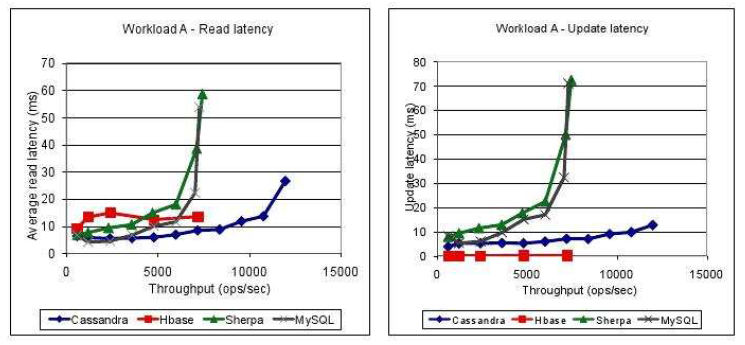
\includegraphics[width=.9\textwidth]{img/cargaA.png}
	\caption{Análise - Carga de trabalho A}
	\label{img:cargaA}
\end{figure}

\begin{figure}[ht]
	\centering
	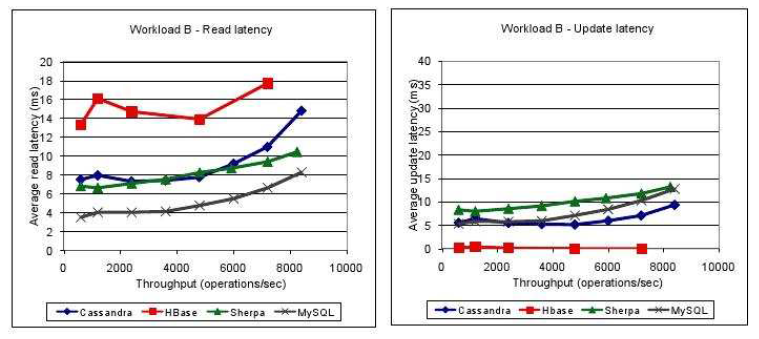
\includegraphics[width=.9\textwidth]{img/cargaB.png}
	\caption{Análise - Carga de trabalho B}
	\label{img:cargaB}
\end{figure}

Como resultados da análise, na carga de trabalho A podemos observar que o Cassandra e o HBase são ótimos para escrita tendo um maior desempenho e menor latência, porem o HBase é inferior no quesito leitura. Já na carga de trabalho B os resultados foram os mesmos. O banco de dados Sherpa apresentou um ótimo desempenho em média.

Como resultado ainda foi possível constatar que que o banco de dados relacional teve uma performance constante porém atingiu uma maior latência se comparado aos NoSQL estudados. Como conclusão do estudo de caso foi considerado que os bancos de dados NoSQL tiveram maior performance que o relacional na maioria dos casos.

\section{Conclusão}
\label{sec:conclusao}

Deste modo os Bancos de Dados NoSQL surgiram como um alternativa aos Banco de dados Relacionais, trazendo novos conceitos principalmente o de flexibilidade e escalabilidade horizontal, não presentes nos Relacionais, sendo que o NoSQL vem como uma alternativa e não como uma substituição do Relacional, mas sim, como uma alternativa que visa dar um melhor desempenho para algumas aplicações que não precisam seguir estritamente o Relacional, ou seja, a finalidade está em otimizar em detrimento de alguns aspectos de consistencia propriamente dito, pois nem todas as aplicações precisam de consitência elevada em todo momento, algumas aplicações precisam de maior liberdade para trabalhar com seus dados, pois tem propósistos diferentes para utiliza-los.

Outro aspecto importante é que embora existam poucos estudos que realmente realizam a comparação entre os tipos de banco de dados NoSQL e relacional, podemos ressaltar através do estudo de caso apresentado a força com o qual os banco de dados não-relacionais estão invadindo o mercado, fazendo com que uma das grandes marcas do mundo o Facebook invista na tecnologia criando o Cassandra, mas não somente invista no ponto de vista de desenvolvimento, como também na utilização de banco de dados não-relacionais em sua rede social.

\bibliographystyle{sbc}
\bibliography{sbc-template}

\end{document}
